\chapter{Proposed Approach}
\label{ch:prop}

The contributions of this project can be seen as two main categories of research work. The first set was accomplished in the beginning phase of this project: behavioral and explicit error propagation through the implementation of the Safety Annex for AADL~\cite{Stewart17:IMBSA,stewart2020safety}. The remaining pieces of this research provide the bulk of the contribution and consist of the compositional generation of minimal cut sets through the transformation of inductive validity cores and using the fault tree generated by this transformation to compute the probability of a safety property violation. 

The usage of the terms error, failure, and fault are defined in ARP4754A and are described here for ease of understanding~\cite{SAE:ARP4754A}. An \textit{error} is a mistake made in implementation, design, or requirements. A \textit{fault} is the manifestation of an error and a \textit{failure} is an event that occurs when the delivered service of a system deviates from correct behavior. If a fault is activated under the right circumstances, that fault can lead to a failure. The term \textit{error propagation} is used to refer to the propagation of the corrupted state caused by an active fault.

\section{The Safety Annex and Fault Modeling}
\subsection{Implementation}
The Safety Annex is written in Java as a plug-in for the OSATE AADL toolset, which is built on Eclipse.  It is not designed as a stand-alone extension of the language, but works with behavioral contracts specified using the AGREE AADL annex~\cite{NFM2012:CoGaMiWhLaLu}. 
The architecture of the Safety Annex is shown in Figure~\ref{fig:plugin-arch}.

\begin{figure}[h!]
	\begin{center}
		%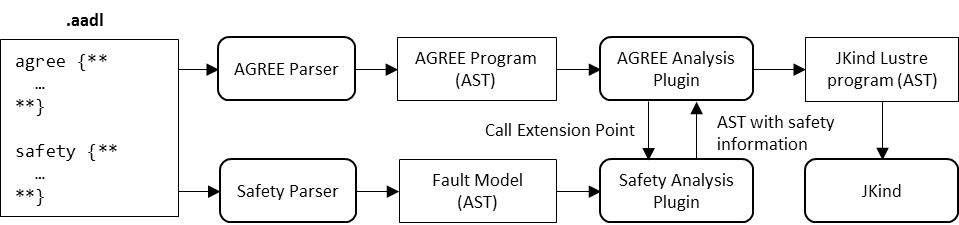
\includegraphics[trim=0 400 430 0,clip,width=0.85\textwidth]{images/arch.png}
		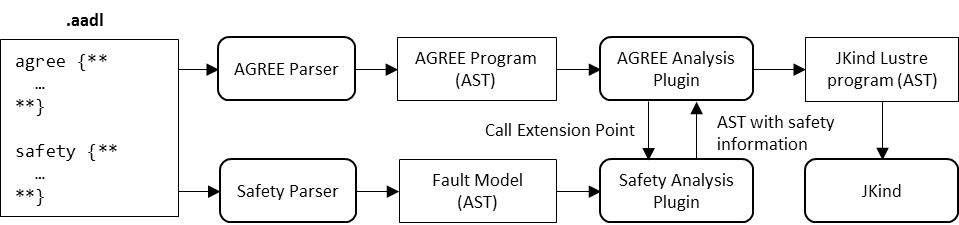
\includegraphics[width=\textwidth]{images/arch.png}
	\end{center}
	%\vspace{-0.1in}
	\caption{Safety Annex Plug-in Architecture}
	\label{fig:plugin-arch}
	%\vspace{-0.1in}
\end{figure}

AGREE contracts are used to define the nominal behaviors of system components as guarantees that hold when assumptions about the values the component's environment are met. When an AADL model is annotated with AGREE contracts and the fault model is created using the Safety Annex, the model is transformed through AGREE into a Lustre model~\cite{Halbwachs91:IEEE} containing the behavioral extensions defined in the AGREE contracts for each system component. 

When an AADL model is annotated with AGREE contracts and the fault model is created using the Safety Annex, an extension point between AGREE and the Safety Annex allows the fault information to be added to the AGREE \textit{abstract syntax tree} (AST). This extended model AST is then translated into Lustre~\cite{Halbwachs91:IEEE}, a synchronous dataflow language used by JKind, an infinite-state model checker for safety properties~\cite{2017arXiv171201222G}. 

The fault model extension of the contracts written in AGREE allows faults to modify the behavior of component outputs. An example of a portion of a nominal AGREE node written in Lustre and its extended contract is shown in Figure~\ref{fig:lustre}. The left column of the figure shows the nominal Lustre pump definition with an AGREE contract on the output; and the right column shows the additional local variables for the fault (boxes 1 and 2), the assertion binding the fault value to the nominal value (boxes 3 and 4), and the fault node definition (box 5). Once augmented with fault information, the AGREE model follows the standard translation path to the model checker JKind. 

\begin{figure}[h!]
	\hspace*{-2cm}
	%\vspace{-0.1in} 
	\begin{center}
		%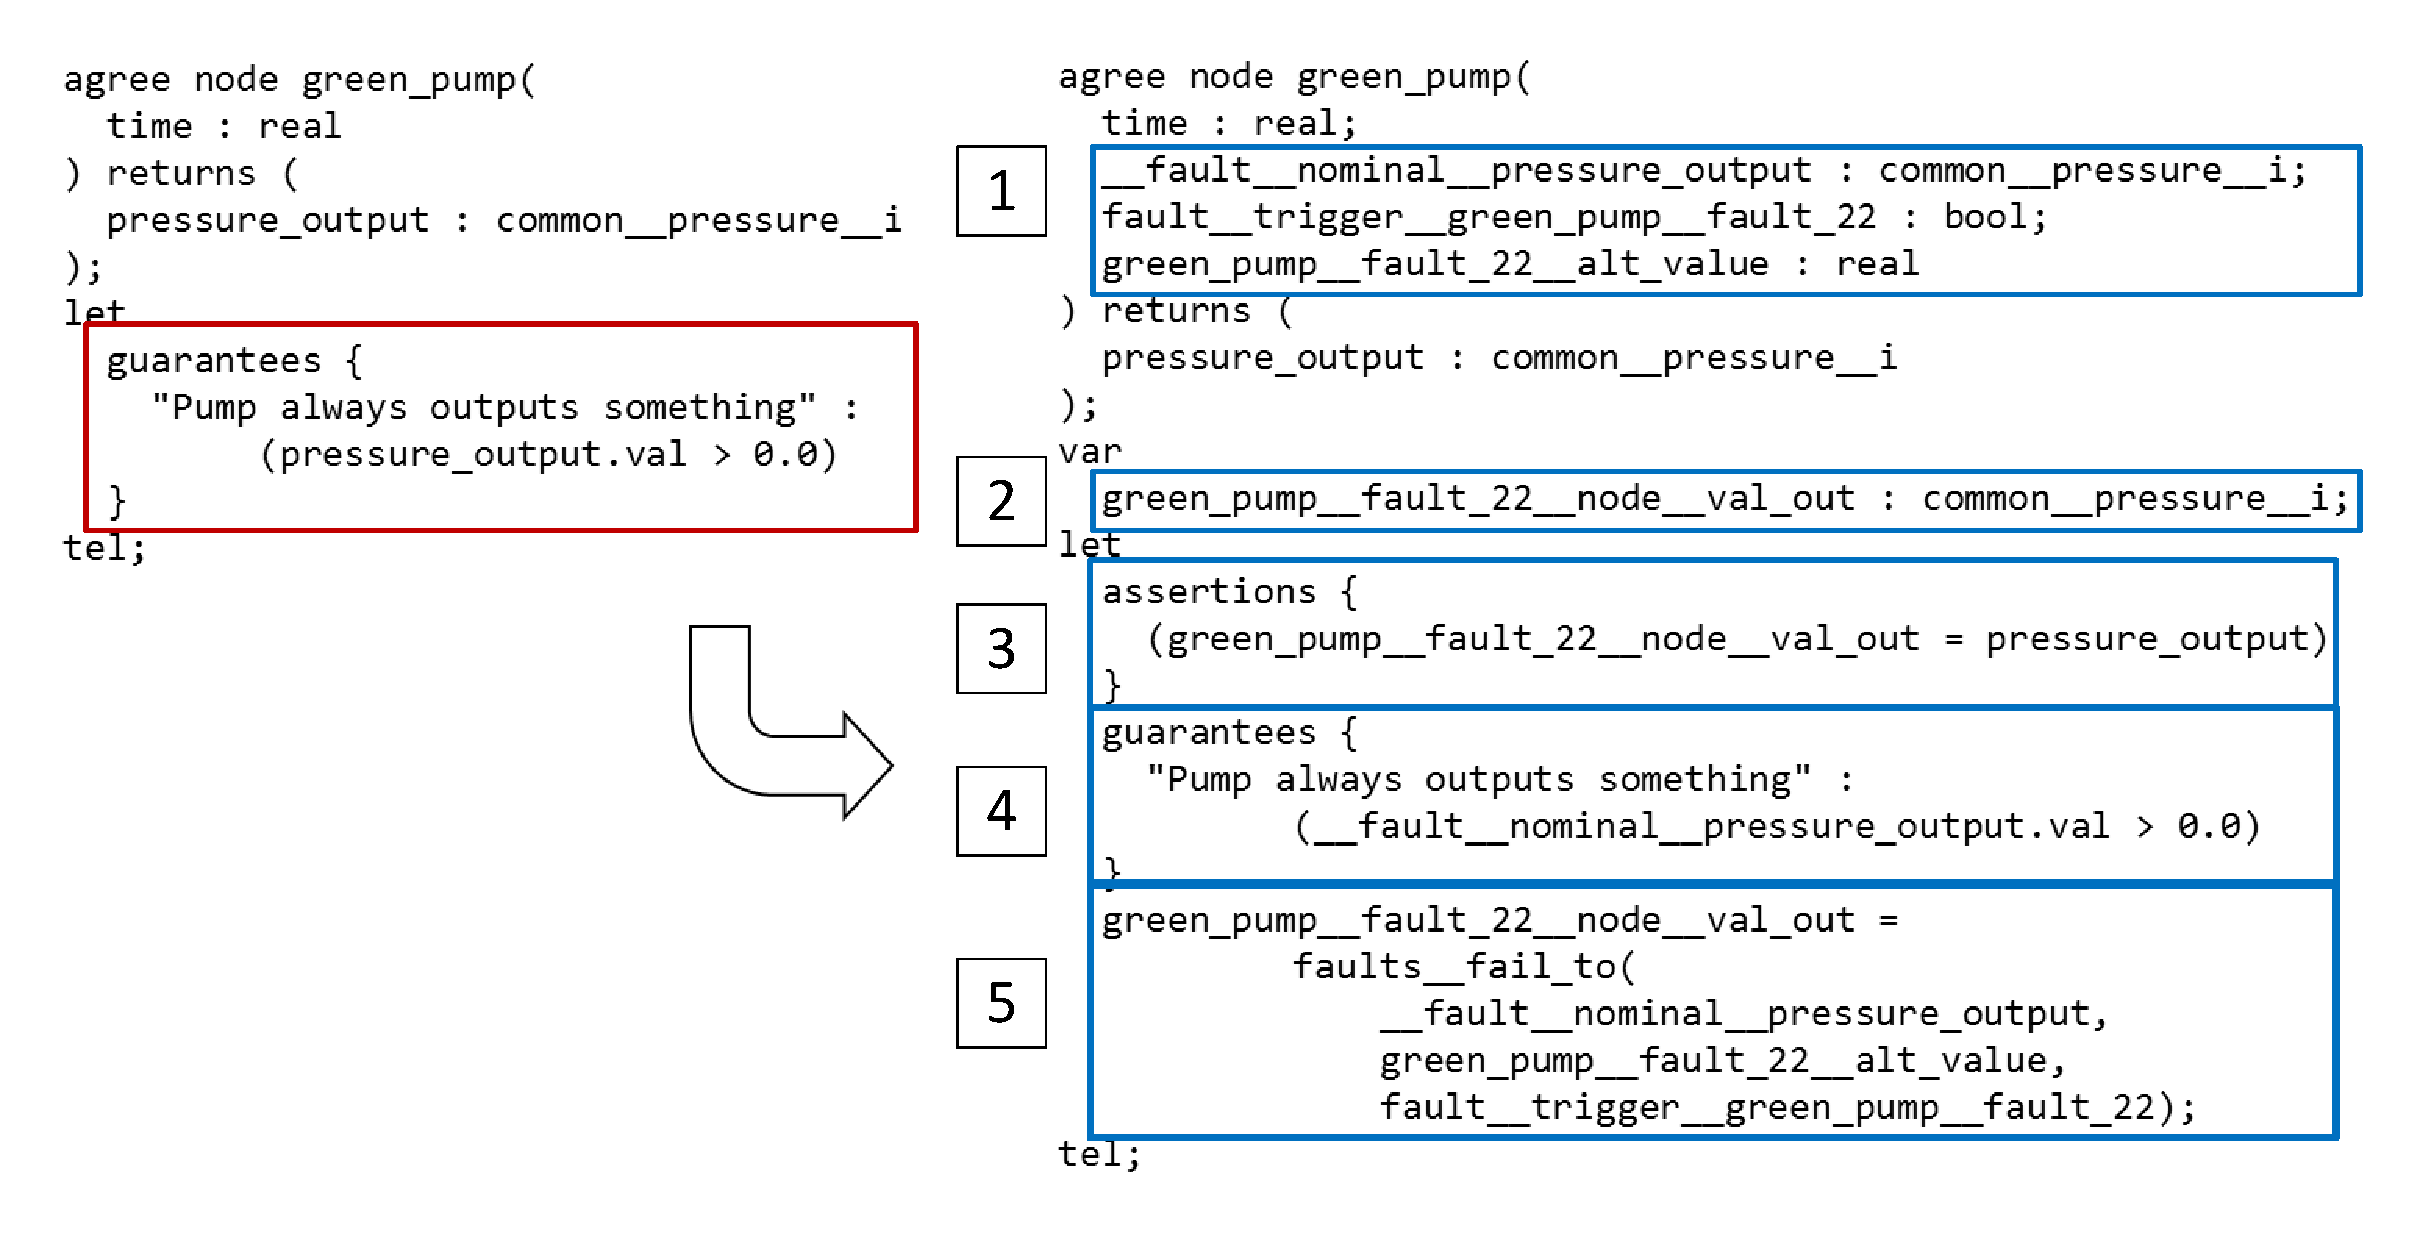
\includegraphics[trim=0 690 -10 70,clip,width=1.5\dimexpr\textwidth-2cm\relax]{images/lustre.pdf}
		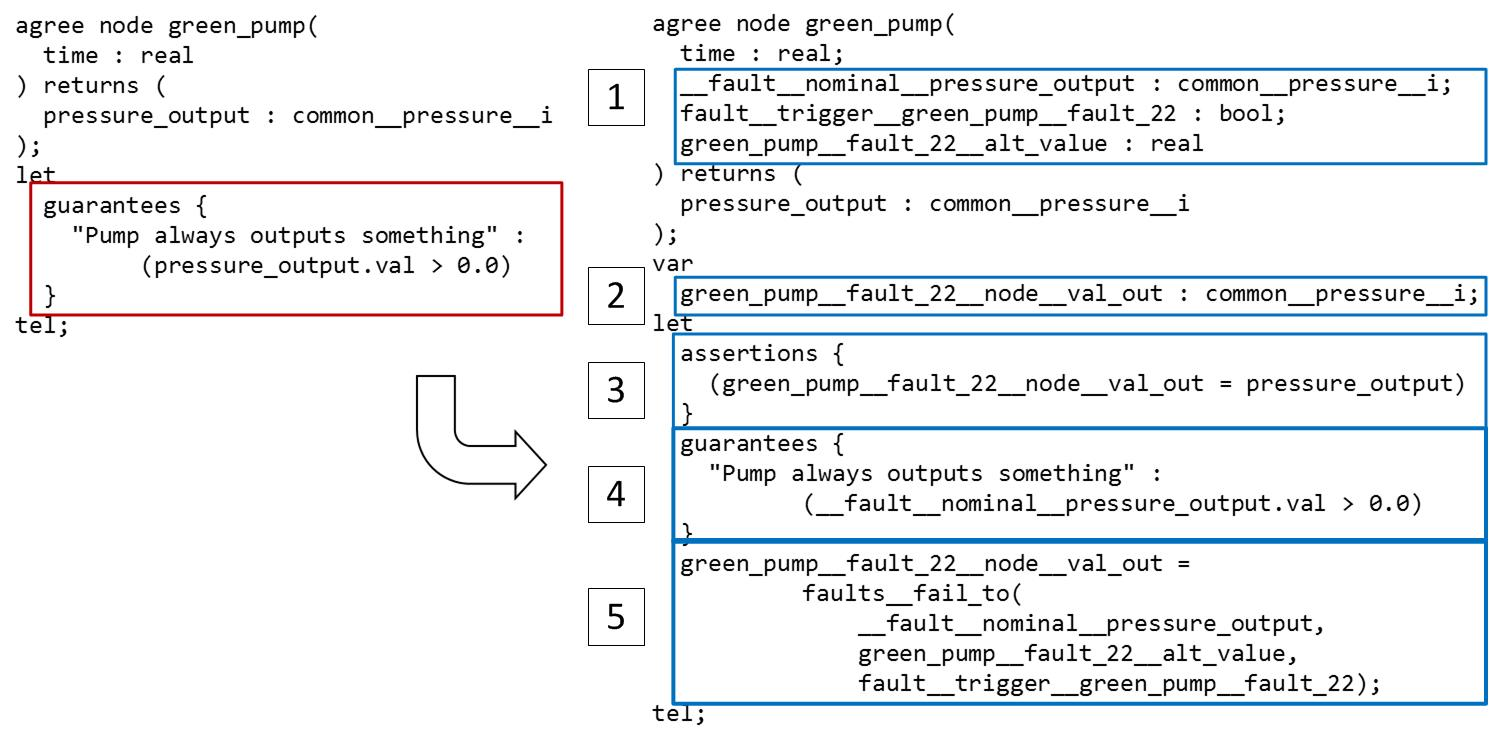
\includegraphics[scale=0.3]{images/lustre.jpg}
		%\caption{Nominal AGREE node and its extension with faults}
		\caption{Nominal AGREE Node and Extension with Faults}
		\label{fig:lustre}
	\end{center}
	%\vspace{-0.1in}
\end{figure}


\subsection{The Sensor System}
\label{sec:sensorExample}
An example is a helpful guide to illustrate the Safety Annex. A simple sensor system is shown in Figure~\ref{fig:sensorSys}. The top level of the system takes two inputs; environmental pressure and temperature. Each subsystem monitors its corresponding input and will send an shutdown command if the input surpasses some threshold. Each subsystem consists of three sensors. Each subsystem's output is regulated by a majority voter; thus, if the majority of sensors in a subsystem report high temperature (or pressure), the shutdown command is sent. 

\begin{figure}[h]
	%\vspace{-0.956in}
	\centering
	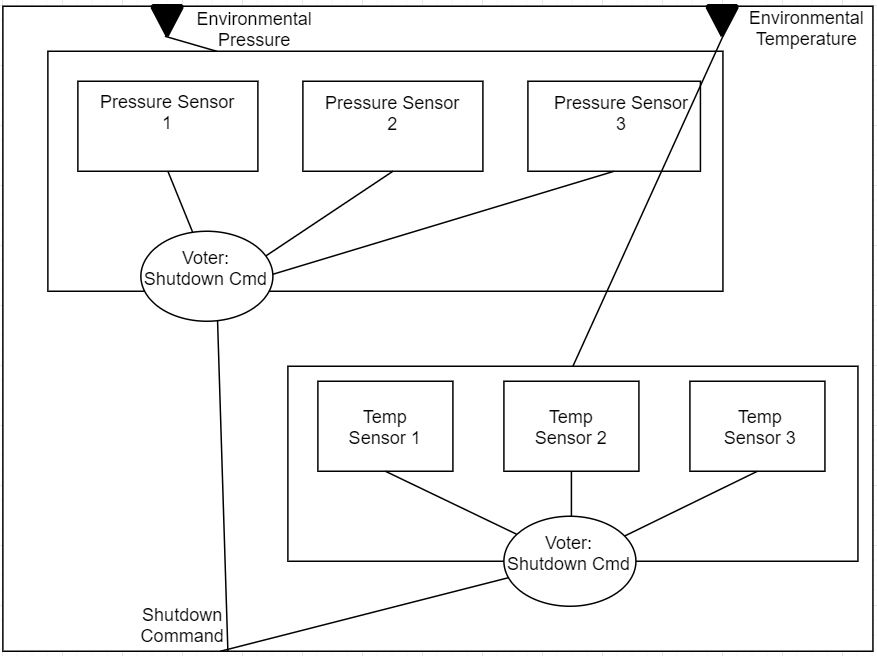
\includegraphics[width=0.6\textwidth]{images/two_sensors.PNG}
	%\vspace{-0.4in}
	\caption{A Simple Sensor System}
	\label{fig:sensorSys}
\end{figure}

This example will be referenced intermittently throughout this document.  

\subsection{The Safety Annex for the Sensor System}
In short, the Safety Annex allows users to describe faults and connect them to AADL component outputs. Within the AADL component instance model, an annex is added which contain the fault definitions for the given component. The flexibility of the fault definitions allows the user to define numerous types of fault \textit{nodes} by utilizing the AGREE node syntax. An example of the AGREE and Safety Annexes defined on a pressure sensor in the sensor system is shown in Figure~\ref{fig:annexes}. 
\begin{figure}[h]
	%\vspace{-0.956in}
	\centering
	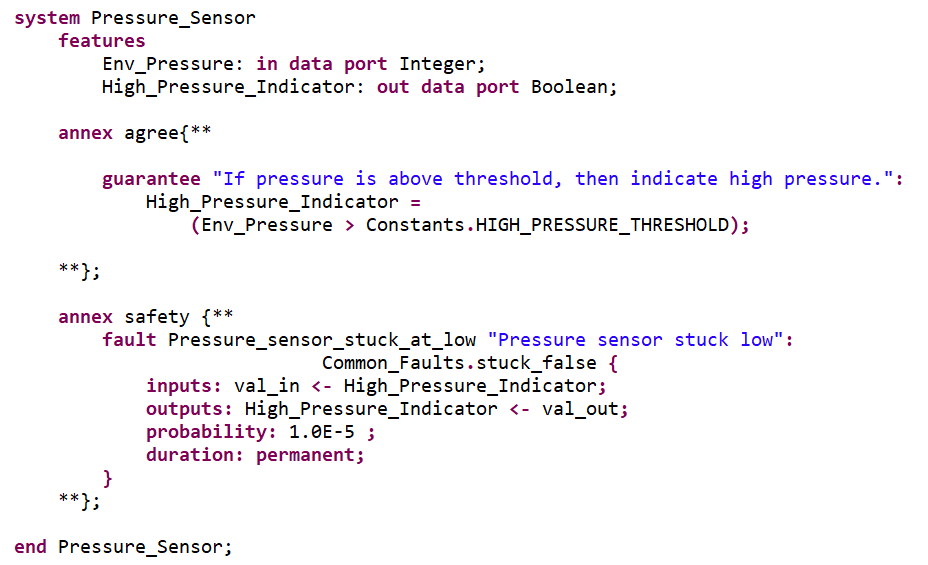
\includegraphics[width=0.7\textwidth]{images/sensorAnnexes.PNG}
	%\vspace{-0.4in}
	\caption{A Pressure Sensor and the AGREE and Safety Annexes}
	\label{fig:annexes}
\end{figure}
The fault definition connects to a \textit{fault node} that is defined in Figure~\ref{fig:node} (the reference to this fault node is seen in the syntax of the fault definition in Figure~\ref{fig:annexes}: \texttt{Common\_Faults.stuck\_false}). The fault node, \texttt{stuck\_false}, restricts the output to false, even when the pressure is higher than the threshold.
\begin{figure}[h]
	%\vspace{-0.956in}
	\centering
	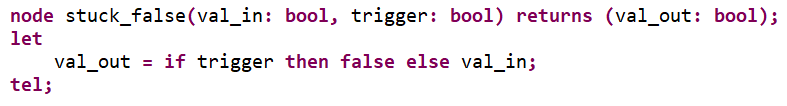
\includegraphics[width=0.6\textwidth]{images/sensorNode.PNG}
	%\vspace{-0.4in}
	\caption{A Fault Node Definition}
	\label{fig:node}
\end{figure}

When a fault is activated by a trigger condition, the fault node outputs a value which overrides the component's nominal output value. The faulty behavior may violate the contracts of other components in the system, including assumptions of downstream components. The impact of a fault is shown by counterexamples returned by the model checker when fault analysis is run on the model.

The fields of a fault definition are shown in Figure~\ref{fig:annexes} and are described for clarity.
\begin{itemize}
\item \textbf{Fault node statement}: This is seen as \texttt{Common\_Faults.stuck\_false} in the figure and refers to a file of fault node definitions (\texttt{Common\_Faults}) containing commonly used faults such as stuck false, stuck true, fail to, or in this case \texttt{stuck\_false}. This provides the node definition in the Lustre code.
\item \textbf{Input}: The inputs state which values from the component are passed into the node definition. In this case, the nominal component (pressure sensor) output \texttt{High\_Pressure\_Indicator} is passed into the node parameter \texttt{val\_in}. 
\item \textbf{Output}: The output from the fault node is designated to an AADL component feature, essentially overwriting it if the fault is active. In this case, the node's output will be the pressure sensor output: \textit{High\_Pressure\_Indicator}. 
\item \textbf{Probability}: This field specifies the probability of occurrence for this fault. This is required for probabilistic analysis.
\item \textbf{Duration}: When a fault becomes active, it is designated as a permanent fault. 
\end{itemize}

\subsection{Modeling Dependent Faults}
%Within the AADL component instance model, the Safety Annex is added which contain the fault definitions for the given component. When a fault is activated by its specified triggering conditions, it modifies the output of the component. This faulty behavior may violate the contracts of other components in the system, including assumptions of downstream components. 
The impact of a fault is computed by the AGREE model checker when the safety analysis is run on the fault model and thus determined implicitly; the error propagation is not explicitly defined as in other closely related tools~\cite{EMV2,compass30toolset}. However, failures in hardware (HW) components can trigger behavioral faults in the system components that depend on them. This makes it beneficial to allow for explicit error propagation and the notion of dependencies in the fault model. For example, a CPU failure may trigger faulty behavior in the threads bound to that CPU or a failure in one HW component may trigger failure in other HW components located nearby, such as overheating, fire, or an explosion in the containment location. The Safety Annex provides the capability to explicitly model the impact of hardware failures on other faults, behavioral or non behavioral. 

Users specify dependencies between the HW component faults and faults that are defined in other components, either HW or SW. The hardware fault then acts as a trigger for its dependencies. This allows for propagation from the faulty HW component to the components that rely on it, affecting the behavior on the outputs of the affected SW components. Within the Lustre implementation, this corresponds to a statement linking the active fault to all dependent faults. Thus, if the triggering fault is active, so are all dependencies.

\section{Verification Capabilities in the Face of Component Failures}
When performing safety analysis, it is useful to be able to restrict the number of failed components in terms of a maximum number or a probabilistic computation. Instead of allowing the Lustre fault activation assignments to remain unrestricted, statements can be added to the Safety Annex that specify the type of analysis to be run. This is either \textit{maximum fault analysis} or \textit{probabilistic threshold analysis}. 

The fault analysis statement (also referred to as the fault hypothesis) resides in the AADL system implementation that is selected for verification. This may specify either a maximum number of faults that can be active at any point in execution (Figure~\ref{fig:hypothesisMaxN}) or that the only faults to be considered are those whose probability of simultaneous occurrence is above some probability threshold (Figure~\ref{fig:hypothesisProb}).

\begin{figure}[h!]
	\vspace{-0.1in}
	\begin{center}
		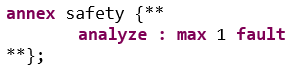
\includegraphics[width=0.4\textwidth]{images/hypothesisMaxN.png}
	\end{center}
	\vspace{-0.1in}
	\caption{Max N Faults Analysis Statement}
	\label{fig:hypothesisMaxN}
\end{figure} 

\begin{figure}[h!]
	\vspace{-0.1in}
	\begin{center}
		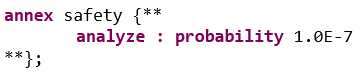
\includegraphics[width=0.5\textwidth]{images/hypothesisProb.png}
	\end{center}
	\vspace{-0.1in}
	\caption{Probability Analysis Statement}
	\label{fig:hypothesisProb}
\end{figure}

Tying back to the fault tree analysis in traditional safety analysis, the former is analogous to restricting the minimal cut sets to a specified maximum number of terms, and the latter is analogous to restricting the minimal cut sets to only those whose probability is above some set value. In the former case, we assert that the sum of the active faults is at or below some integer threshold.  In the latter, we determine all combinations of faults whose probabilities are above the specified probability threshold, and describe this as a proposition over fault activation literals. 
%
Active faults are divided into two categories: independently active (activated by its own triggering event) and dependently active (activated when the faults they depend on become active). The top level fault hypothesis applies to independently active faults. Faulty behaviors augment nominal behaviors whenever their corresponding faults are active (either independently active or dependently active).

\subsection{Maximum Fault Analysis}
The max fault hypothesis specifies a maximum number of faults that can be active at any point in execution. This is analogous to restricting the minimal cut sets to a specified maximum number of terms in the fault tree analysis in traditional safety analysis. In implementation (i.e., the translated Lustre model feeding into the model checker), we assert that the sum of the fault activation literals assigned to \textit{true} is below some integer threshold. This can be seen in Figure~\ref{fig:count} with maximum fault count set at 3.
\begin{figure}[h]
	%\vspace{-0.1in}
	\begin{center}
		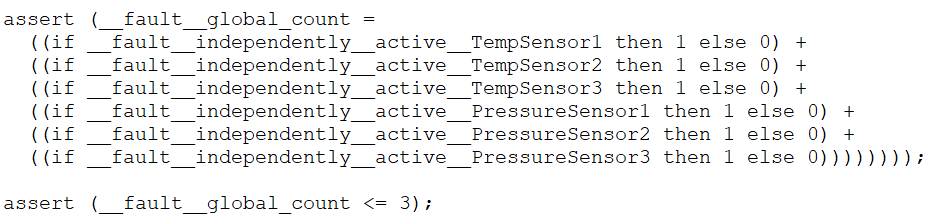
\includegraphics[width=0.7\textwidth]{images/assertCount.PNG}
	\end{center}
	%\vspace{-0.1in}
	\caption{Lustre Statement for Fault Count}
	\label{fig:count}
\end{figure}
While solving the satisfiability problem, JKind will iterate through the possible combinations given the restriction of the hypothesis statement. If the system with respect to a certain safety property is found to be UNSAT, a counterexample showing the trace of the system (including active faults) is given to the user. 

When running the analysis compositionally, JKind employs a top-down approach; it attempts to prove the top-level requirements using the contracts of the direct subcomponents, then it moves to the next layer down, and so on. If using maximum N fault analysis compositionally, the results pertain only to the current level of analysis.

In the traditional safety assessment process, safety analysts require information regarding single points of failure on specific components or even system wide. The Safety Annex supports this need and the detailed counterexamples can provide important insight into the system development process. 

\subsection{Probabilistic Threshold Analysis}
The grammar of the Safety Annex allows for a probabilistic assignment to a fault definition as shown in Figure~\ref{fig:annexes}. The \textit{probabilistic fault hypothesis} specifies that only faults whose probability of simultaneous occurrence is above some probability threshold should be considered. In the implementation, we determine all combinations of faults whose probabilities are above the specified probability threshold and describe this as a proposition over the fault activation literals. If the probability of a combination of faults is less than the designated top level threshold, these faults may be activated and the behavioral effects can be seen through a counterexample.  

To perform this analysis, it is assumed that the faults occur independently. Algorithm 1 describes this process. First, all faults are removed from consideration that are too unlikely given the probability threshold. The remaining faults are arranged in a priority queue $\mathcal{Q}$ from high to low. Take the fault with highest probability from the queue (step 5) and attempt to combine the remainder of the faults in $\mathcal{R}$ (step 7). If this combination is lower than the threshold (step 8), then we do not take into consideration this set of faults and instead remove the tail of the remaining faults in $\mathcal{R}$. %The reason we can do this is because of the arrangement in priority queue from highest to lowest value. If this combination is below threshold, certainly any other combination of these faults with one of lesser value in the priority queue will also be below threshold. 
 
In this calculation, we assume independence among the faults, but in the Safety Annex it is possible to define dependence between faults using a fault propagation statement. After the possible fault combinations are computed using Algorithm 1, the triggered dependent faults are added to the combination as appropriate while ignoring their respective probabilities.

\begin{algorithm}[H]
	% \KwData{this text}
	% \KwResult{how to write algorithm with \LaTeX2e }
	$\mathcal{F} = \{\}$ : fault combinations above threshold \;
	$\mathcal{Q}$ : faults, $q_i$, arranged with probability high to low \;
	$\mathcal{R} = \mathcal{Q}$ , with $r \in \mathcal{R}$\;
	\While{$\mathcal{Q} \neq \{\} \land \mathcal{R} \neq \{\}$ }{
		$q =$ removePriorityElement($\mathcal{Q}$) \;
		\For{$i=0:|\mathcal{R}|$}{
			$prob = q \times r_i$ \;
			\eIf{prob $<$ threshold}{
				removeTail($\mathcal{R}, i:|\mathcal{R}|$)\;
			}{
				add($\{q, r_i\}, \mathcal{Q}$)\;
				add($\{q, r_i\}, \mathcal{F}$)\;
			} % end if else
		} % end for
	} % end while
	\caption{Monolithic Probability Analysis}
\end{algorithm}

Often it is the case that safety properties contain probabilistic thresholds that must be analyzed during the safety assessment process. This type of fault hypothesis statement and the associated fault analysis supports these requirements.

\section{Generation of Minimal Cut Sets from MIVCs}
\subsection{The General Idea}
As was previously explained, the MIVCs (Minimal Inductive Validity Cores) are MUSs (Minimal Unsatisfiable Subsets) of a constraint system. The MCSs (Minimal Correction Sets) can be obtained from all MUSs by generating the hitting sets of all MUSs. Thus, the All-MIVC algorithm produces all MUSs and the hitting set algorithm can transform these into MCSs. If the constraint system is defined to take into account faults, these MCSs can be transformed into MinCutSets. 

Recall that a constraint system is an ordered set of abstract constraints over a set of variables. In the case of a nominal model augmented with faults, a constraint system can be defined as follows. Let $F$ be the set of fault activation literals and $G$ be the set of component contracts (guarantees). 

\begin{definition}A constraint system $C = \{C_1,C_2,...,C_n\}$ where for $i \in \{1,...,n\}$, $C_i$ has the following constraints for any $f_j \in F$ and $g_k \in G$ with regard to the top level property $P$: 
\begin{center}
$C_i \in \left\{ \begin{array}{ll}
	f_j :&  false\\
	g_k :& true\\
	P :& false\\
\end{array}\right.$	
\end{center}
\label{def:constraintsystem}
\end{definition}

The All-MIVC algorithm collects all minimal unsatisfiable subsets of a given transition system in terms of the \textit{negation} of the top level property~\cite{Ghassabani2017EfficientGO,bendik2018online}. Assuming that the nominal model proves (no faults are active), it is not surprising that the guarantees (constrained to \textit{true}) and the negation of the safety property is UNSAT. The MUSs are the minimal explanation of the infeasibility of this constraint system; equivalently, these are the minimal sets of model elements necessary for proof of the safety property.

We utilize this algorithm by providing not only component contracts constrained to \textit{true} as model elements, but also fault activation literals constrained to \textit{false}, i.e. the faults are inactive. Thus the resulting MIVCs (MUSs) will contain the required contracts and constrained fault activation literals necessary to prove the safety property. 

Because of the duality between MUSs and MCSs, all MCSs can be obtained by finding the hitting sets. The MCS can be seen to correct the infeasibility of the constraint system and provides the minimal such correction. By removing the constraints from $C$ that are found in any MCS, $C$ becomes satisfiable. In terms of our constraint system with fault activation literals, by \textit{activating} the faults in the MCS and \textit{violating} the contracts in the MCS, we can prove the \textit{negation} of the property $P$. If the contracts in the MCS are replaced with the faults that cause its violation, the MCS is transformed into a MinCutSet.\\

\textbf{The Steps of Transformation from MUS to MinCutSet}
\begin{enumerate}
\item Redefine constraint system by adding fault activation literals to the constraint system used by the All-MIVC algorithm. %The MIVC algorithm proceeds compositionally, so the changes to the constraint system must also be factored in on a per-layer basis. For the leaf levels of the system, we add all fault activation literals as model elements for consideration. For all other layers, we provide the guarantees of the layer beneath and if the layer beneath is 
\item Transform the MUSs (MIVCs) into MCSs by use of a hitting set algorithm~\cite{murakami2013efficient,gainer2017minimal}. 
\item Replace all contracts in the MCSs by the faults that cause their violation (MinCutSets for that contract). 
\end{enumerate}

\subsection{Illustrative Example}
Using the sensor system described in Section~\ref{sec:sensorExample}, this transformation can be more easily understood. The top-level safety property of the system states that a shutdown occurs when and only when it should: 
\begin{center}
    ($temp\_input > threshold$) $\lor$ ($pressure\_input > threshold$)\\
    $\iff Shutdown$
    
\end{center}

The property of each sensor subsystem states that when the majority of sensors report high, denoted as $out_{si}$ for sensor $si$, a shutdown command is sent:
\begin{center}
    $majority\_vote(out_{s1}, out_{s2}, out_{s3}) \iff Shutdown$
    
\end{center}

Each sensor has a behavioral property stating that if the environmental input is high, the shutdown command is sent: 
\begin{center}
    $(environment > threshold) \iff Shutdown$
    
\end{center}

A fault is defined on each of the sensors which when active, causes the sensors to fail low (the environmental input is high, but they do not send a shutdown command). It is easy to see that this system is resilient to a single fault anywhere due to the majority voting mechanism. \\

\textbf{Leaf Level}: To illustrate the MIVC to MinCutSet transformation, we start with a leaf level of the system: a pressure sensor, $p1$. (Note: The MIVC algorithm proceeds in a top-down fashion, but for clarification in the example, we look at the results in a bottom-up approach.)  In this layer, the MIVC algorithm treats the sensor guarantee, $g_{p1}$, as the property of interest:
\begin{center}
    $g_{p1} : (environment > threshold) \iff Shutdown$
\end{center}
and the model elements provided to the MIVC algorithm consist of only fault activation literals for this leaf component constrained to \textit{false}; we call the fault on $p1$, $f_{p1}$. Thus, the constraint system for this layer is: 
\begin{center}
    $C_{leaf} = \{\neg f_{p1} \neg g_{p1}\}$
\end{center}

The MIVC algorithm returns all MIVCs for this constraint system, $MIVC = \{\{\neg f_{p1}\}\}$, of which there is only one: in order for this leaf level guarantee to hold, the fault must be constrained to false. 

The hitting set algorithm finds that the set $\{\neg f_{p1}\}$ sufficiently 'hits' all MIVCs and this is our MCS. This means that if the constraint is removed from $f_{p1}$ in $C$, our constraint system is satisfiable. Thus, the MinCutSet for $\neg g_{p1}$ is $\{f_{p1}\}$, and in the same manner, we find the MinCutSets for $g_{p2}, g_{p3}$ and the guarantees for the temperature sensors. \\

\textbf{Mid Level}: For the mid-level pressure system, $P$, the guarantee of interest is: 
\begin{center}
    $g_P : majority\_vote(out_{p1}, out_{p2}, out_{p3}) \iff Shutdown$
\end{center}
and can be also written as: 
\begin{center}
    $g_P: ((out_{p1} \land out_{p2}) \lor (out_{p1} \land out_{p3}) \lor (out_{p2} \land out_{p3})) \iff Shutdown$
\end{center}

The constraint system looks only at the supporting guarantees (one level below) and any fault literals in the current level. Thus, the constraint system is: 
\begin{center}
    $C = \{g_{p1}, g_{p2}, g_{p3}, \neg g_P\}$
\end{center}

The resulting MIVCs are: $\{\{g_{p1}, g_{p2}\}, \{g_{p1}, g_{p3}\}, \{g_{p2}, g_{p3}\}\}$. If any pairwise combination of guarantees hold, then the property $g_P$ holds, i.e. the shutdown command is sent. The hitting set algorithm determines all sets whose intersection with all MIVCs are nonempty. In this case, they are equivalent to the MIVCs. 

Since MinCutSets only contain faults, a replacement must be made between the guarantees found in the MCSs and the faults that cause the violation of these guarantees. We know those faults due to the processing done at the leaf level; after replacement, we obtain the MinCutSets for $\neg g_P$: $\{\{f_{p1}, f_{p2}\}, \{f_{p1}, f_{p3}\}, \{f_{p2}, f_{p3}\}\}$.\\

\textbf{Top Level}: The top level property is: $(temp\_input > threshold)$ $\lor$ $(pressure\_input > threshold) \iff Shutdown$, and requires guarantees from both the temperature and pressure subsystems, $g_P$ and $g_T$ respectively. The resulting MIVCs are: $\{\{g_P\}, \{g_T\}\}$. This is also equivalent (in this case) to the MCSs generated through the hitting set algorithm. Replacement of these contracts with the faults that cause their violation produces all MinCutSets for the top level event (violation of the top level safety property). This is: any combination of two faults occurring in either the temperature or the pressure sensor systems will result in violation of the safety property. \\

The example should suffice to show the basic outline of the algorithm. The proofs showing that this transformation is logically valid will be provided in the dissertation and the algorithms will be implemented in the Safety Annex.  


\section{Compositional Probabilistic Computations}
Safety analysis techniques aim at demonstrating that the system meets the requirements necessary for certification and use in the presence of faults. In many domains, there are two main steps to this process: (1) the generation of all minimal cut sets (MinCutSets), i.e. the minimal set of faults that lead to a violation of the top level property (known as a \textit{top-level event} or TLE) and (2) the computation of the corresponding fault probability, i.e. the probability of reaching the TLE, given probabilities for the faults in the system. 

The probability of the TLE is used to find the likelihood of the safety hazard that it represents. While evaluation of the fault model with a given probabilistic threshold does provide information on the safety hazards, it is also informative and desirable to find the overall probability of the occurrence of a hazard. 

Such computations can be carried out by leveraging the logical formula represented by the disjunction of all MinCutSets which are in turn conjunctions of their constituents. 

Given a set of MinCutSets and a mapping $\mathcal{P}$ that gives the probability of the basic faults in the system $f_i$, it is possible to compute the probability of occurrence of the TLE. Assuming that the basic faults are independent, the probability of a single MinCutSet, $\sigma$ is given by the product of the probabilities of its basic faults:
\begin{center}
    \begin{equation*}\mathcal{P}(\sigma) = \prod_{f_i \in \sigma} \mathcal{P}(f_i) 
    \end{equation*}    
\end{center}

For a set of MinCutSets, $S$, the probability can be computed using the following recursive formula:

\begin{center}
    $\mathcal{P}(S_1 \cup S_2) = \mathcal{P}(S_1) + \mathcal{P}(S_2) - \mathcal{P}(S_1 \cap S_2)$
\end{center}

Due to the independence assumption, $\mathcal{P}(S_1 \cap S_2)$ is computed as $\mathcal{P}(S_1) \cdot   \mathcal{P}(S_2)$. Using this technique, it is theoretically possible to compute the overall probability of a TLE given all MinCutSets and an independence assumption, but in the real world of safety analysis this poses some problems, the largest of which is scalability. Given a very large system with many possible faults, it becomes difficult to compute all MinCutSets without pruning of any kind. If one is unable to complete such computations, it is not possible to simply compute the probabilities as described above. 

As previously discussed, it is standard practice to consider cut sets only up to a given cardinality. As the cardinality of the cut sets increase, the likelihood of their occurrence decreases and as the system increases in size, the possible combinations of problematic faults will inevitably increase, at times exponentially. In order to simplify these calculations and address the problem of scalability, MinCutSets up to a certain cardiality are considered. Everything above that is "safely" ignored, and then specific criteria is used to overapproximate the error. The end result of these computations is above the actual probability (i.e. a safe approximation), but close enough to be significant. 

Another drawback to computing an exact probability of the TLE is the problem of model reliability and exactness. For instance, if two groups of engineers each built a model of the same system, the models may not be equivalent; especially in terms of behavioral properties. Since our approach of computing MinCutSets depends on the properties over system components, the calculated top-level probability will change. Different representations of the system will alter the computations.  

As an example, assume that Figure~\ref{fig:probComp1} is a snapshot of a given layer in a system designed by the first group of engineers. Component A has a contract, $G_A$, which is determined by the All-IVC algorithm to depend on a lower level contract, $g_A = a \land b$. $g_A$ will be in the set of IVCs for the contract $G_A$. Assume that only $a$ is required for the proof of $G_A$. 

\begin{figure}[h]
\begin{center}
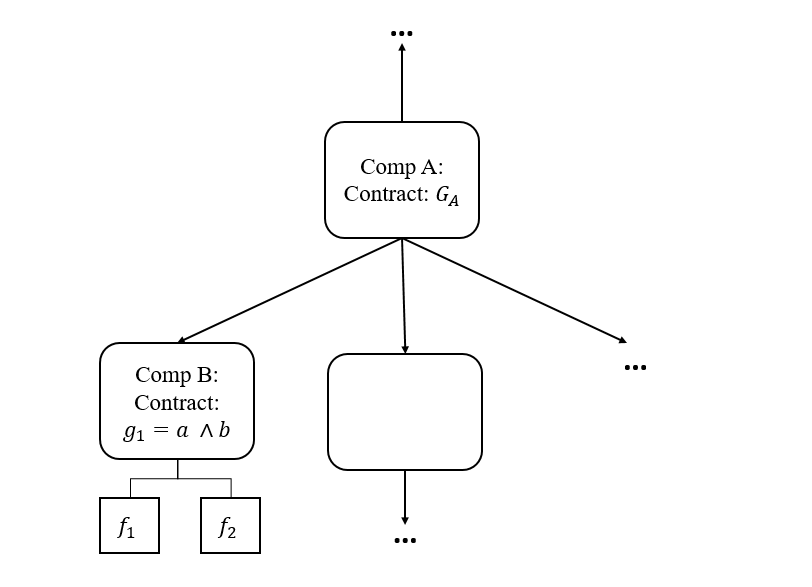
\includegraphics[width=6cm]{images/probComp1.PNG}
\caption{Sample System Contract Part I} \label{fig:probComp1}
\end{center}
\end{figure}

Two faults are defined on component B: $f_1$ violates $a$ and $f_2$ violates $b$. Since each of these faults will violate the contract $g_A$, each of these faults will be found in MinCutSets for $G_A$.

Now assume that Figure~\ref{fig:probComp2} was the system representation built by the second group of engineers. 
\begin{figure}[h]
\begin{center}
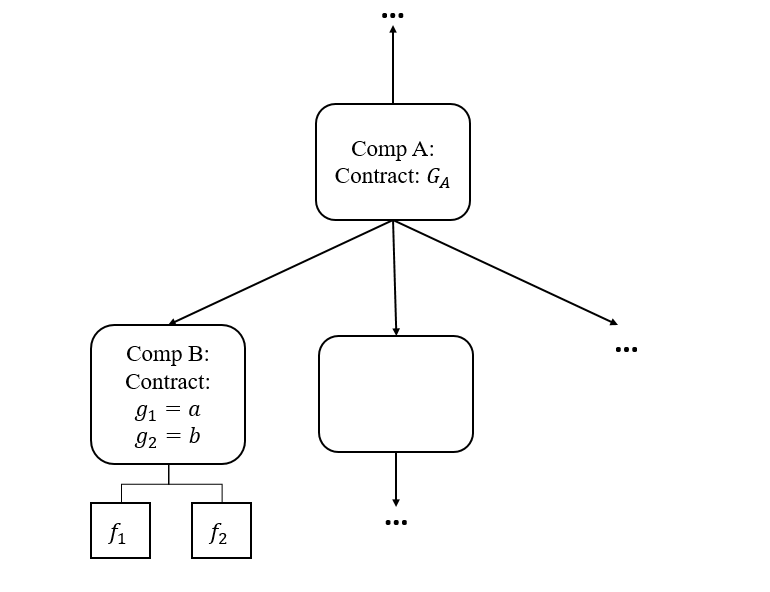
\includegraphics[width=6cm]{images/probComp2.PNG}
\caption{Sample System Contract Part II} \label{fig:probComp2}
\end{center}
\end{figure} 
The basic system structure is the same, but this time they wrote two contracts for component B: $g_1 = a$ and $g_2 = b$. Since $b$ is not required for the proof of $G_A$, only $g_1$ is found in the IVCs for $G_A$ and thus only $f_1$ will be seen in the MinCutSets for this particular contract. 

In this simple example, it is easy to see why a single computation of the top-level probability of a system may be misleading. To this end, we wish to find a way to accurately obtain higher and lower bounds of what the probability is likely to be. 

A lower bound for the probability can be obtained by choosing a maximum cardinality for MinCutSets before computations begin, e.g. assume that cardinalities above $n$ are too unlikely to be significant. This will contribute to better scalability in large systems with numerous possible cut sets. A higher bound is commonly assigned by experts of the system, e.g. around 3 orders of magnitude higher than the lower approximation. 

It would be beneficial to leverage the IVC information to provide both the lower and upper bound approximations and show that these values are significant and trustworthy. 



\section{Evaluation of Results}
The goal of this dissertation is to provide usable and reliable safety assessment artifacts and methodologies that can be implemented on industrial scale systems. Furthermore, the artifacts should shed light on the system organizational hierarchy, interacting components, and problematic faults. This is useful within the assessment process and can provide valuable feedback to engineers on both the safety and development side. 

To this end, we will implement a large scale system model in the aerospace domain and collect the artifacts and other pertinent information derived from this process. We will show how this information can provide feedback to the system engineers and be useful in the certification process. 

The Wheel Brake System (WBS) was initially developed for illustrative purposes by SAE AIR6110~\cite{AIR6110} and has been used in numerous case studies and research into Model-Based Safety Analysis~\cite{Stewart17:IMBSA,DBLP:conf/cav/BozzanoCPJKPRT15,mcmillan2019increasing,cimatti2016temporal,cimatti2018tightening,konrad2016faa}. This model is large enough to assess scalability and provides numerous complex component interactions and behaviors. The AADL version of this model will be annotated with AGREE contracts that accurately describe the behavior of the system components. Faults will be attached to each of the components as per descriptions in AIR6110. The analysis of this approach will address the four main contributions of the Safety Annex: 
\begin{enumerate}
    \item Maximum $n$ fault threshold compositional analysis
    \item Probabilistic threshold monolithic analysis 
    \item Minimal cut set computations (max $n$ and probabilistic threshold)
    \item Probabilistic evaluations and computations
\end{enumerate}

The artifacts generated from each run will be assessed in light of safety assessment and fit into the process as described in Sections \ref{sec:saProcess} and \ref{sec:saProcess2}.

Using other models representative of the aerospace industry, we will explore the necessity of using a shared system model that drives the development and safety processes, and show the fault modeling flexibility of the Safety Annex. 











